\section{THỂ TÍCH}
\subsection{KIẾN THỨC CẦN NHỚ}
\subsubsection{Thể tích khối lăng trụ}
\immini{Thể tích khối lăng trụ bằng diện tích đáy nhân với đường cao của lăng trụ.
\begin{center}
	\fbox{$V=S_{\text{đáy}}\cdot h$}
\end{center}
Trong đó
\begin{listEX}[1]
	\item [\ding{172}] $S_{\text{đáy}}$ là diện tích đáy của khối lăng trụ;
	\item [\ding{173}] $h$ là chiều cao của khối lăng trụ.
\end{listEX}
}{
\begin{tikzpicture}[scale=.6]
	\tkzDefPoints{0/0/A, 2/-2/B, 4/-1.5/C,5/0/D, 1.5/-0.5/H, 1.5/5/z}
	\coordinate (A') at ($(A)+(z)$);
	\coordinate (B') at ($(B)+(z)$);
	\coordinate (C') at ($(C)+(z)$);
	\coordinate (D') at ($(D)+(z)$);
	\tkzDrawPolygon(A',B',C',D')
	\tkzDrawPoints[size=2,fill=black](A',H,B',C',D',A,B,C,D)
	\tkzDrawSegments(A,B B,C C,D A,A' B,B' C,C' D,D')
	\tkzDrawSegments[dashed](A,D A',H)
	\tkzLabelPoints[below right](B')
	\tkzLabelPoints[below](B,H,C)
	\tkzLabelPoints[left](A', A)
	\tkzLabelPoints[right](D,D')
	\tkzLabelPoints[above](C')
	\draw(1.5,1.5)node[right] {$h$};
\end{tikzpicture}\\
\color{violet}\fontsize{9}{0}\selectfont Hình lăng trụ tứ giác $ABCD.A'B'C'D'$}
\subsubsection{Thể tích khối chóp}
\immini{
Ta có thể tích khối chóp bằng một phần ba diện tích đáy nhân với đường cao hình chóp.
\begin{center}
	\fbox{$V_{\text{chóp}}=\dfrac{1}{3}\cdot S_{\text{đáy}}\cdot h$}
\end{center}
Trong đó 
\begin{itemize}
	\item[\ding{172}]$S_{\text{đáy}}=S_{ABCD}$ là diện tích mặt đáy của khối chóp.
	\item[\ding{173}] $h=SH$ là chiều cao của khối chóp.
\end{itemize}}{
\begin{tikzpicture}[scale=0.8, line join=round, line cap=round]
	\tkzInit[xmin=-1.9,xmax=3,ymax=3.2, ymin=-2]
	\tkzDefPoints{0/0/A,-1.3/-1.6/B,2.5/-2/C, 1/-0.4/H, 3/.2/D}
	\coordinate (S) at ($(H)+(0,3)$);
	\tkzDrawPolygon(S,B,C,D)
	\tkzDrawSegments(S,C)
	\tkzDrawSegments[dashed](A,S A,B A,D S,H)
	\tkzLabelPoints[above](S)
	\tkzLabelPoints[below](A,B,C,H)
	\tkzLabelPoints[right](D)
	\draw(0.9,1)node[right] {$h$};
\end{tikzpicture}}

\subsubsection{Thể tích khối chóp cụt đều}
\immini{
Thể tích của khối chóp cụt đều được tính theo công thức
\begin{center}
	\fbox{$V\dfrac{1}{3}\cdot h\cdot (S+S'+\sqrt{S\cdot S'})$}
\end{center}
Trong đó 
\begin{itemize}
	\item[\ding{172}]$S$ là diện tích đáy lớn  của khối chóp cụt đều.
	\item[\ding{172}]$S'$ là diện tích đáy bé  của khối chóp cụt đều.
	\item[\ding{173}] $h=SH$ là chiều cao của khối chóp cụt đều.
\end{itemize}}
{
\begin{tikzpicture}[scale=0.8, font=\footnotesize, line join=round, line cap=round, >=stealth]
	\tkzInit[xmin=-1,xmax=5,ymin=-1.5, ymax=5.5] \tkzClip[space=.1]
	\tkzDefPoints{0/0/A1,2/0/H,1/-1/A2,0/5/x}
	\coordinate (A4) at ($(A1)!2!(H)$);
	\coordinate (A3) at ($(H)-(A1)+(A2)$);
	\coordinate (A5) at ($(A2)!2!(H)$);
	\coordinate (A6) at ($(A3)!2!(H)$);
	\coordinate (S) at ($(H)+(x)$);
	\coordinate (B1) at ($(S)!0.5!(A1)$);
	\coordinate (B2) at ($(S)!0.5!(A2)$);
	\coordinate (B3) at ($(S)!0.5!(A3)$);
	\coordinate (B4) at ($(S)!0.5!(A4)$);
	\coordinate (B5) at ($(S)!0.5!(A5)$);
	\coordinate (B6) at ($(S)!0.5!(A6)$);	
	\coordinate (K) at ($(S)!0.5!(H)$);
	\tkzDrawSegments(A1,A2 A2,A3 A3,A4 B1,B2 B2,B3 B3,B4 B1,A1 B2,A2 B3,A3 B4,A4 B1,B4 B2,B5 B3,B6 B4,B5 B5,B6 B6,B1)
	\tkzDrawSegments[dashed](A1,A4 A4,A5 A5,A6 A6,A1 A3,A6 A2,A5 B5,A5 B6,A6 K,H)
	\node[below right] at (A3) {$S$};
	\node[right] at (B4) {$S'$};
	\draw
	(K)--(H) node[pos=.4,right]{$h$};
\end{tikzpicture}}

\subsection{PHÂN LOẠI, PHƯƠNG PHÁP GIẢI TOÁN}
\begin{dang}{Tính thể tích khối lăng trụ}
	\begin{enumerate}[\iconCH]
		\item \indamm{Phương pháp:}
		\begin{itemize}
			\item Tính diện tích đáy $S_{\text{đáy}}$ và độ dài đường cao $h$ của khối lăng trụ;
			\item Thay vào công thức $V=S_{\text{đáy}} \cdot h$.
		\end{itemize}
		\item \indamm{Các trường hợp đặc biệt:}
		\begin{listEX}[1]
			\item [\ding{172}] Thể tích $V$ của khối hộp chữ nhật có ba kích thước lần lượt $a$, $b$, $c$ là $V=a \cdot b \cdot c$.
			\item [\ding{173}] Thể tích $V$ của khối hộp lập phương có cạnh bằng $a$ là $V=a^3$.
		\end{listEX}
	\end{enumerate}
\end{dang}


\begin{vd}
	\immini{
		Cho lăng trụ đứng $ABC.A'B'C'$ có $AA'=a$, tam giác $ABC$ đều và có cạnh bằng $a$. Tính thể tích của khối lăng trụ đã cho.
		\cham{6}
		}{
		\begin{tikzpicture}[scale=0.7, font=\footnotesize, line join=round, line cap=round, >=stealth]
			\tkzDefPoints{0/0/A,0/2/A',3/0/B, 3/2/B',2/-1/C}
			\tkzDefPointBy[translation = from A to C](A')
			\tkzGetPoint{C'}
			\tkzDrawPoints(B,B',C,C')
			\tkzLabelPoints(B,B',C,C')
			\tkzLabelPoints[left](A',A)
			\tkzDrawSegments(A,C B,C A,A' A',B' B',B A',C' C',C C',B')
			\tkzDrawSegments[dashed](A,B)
			\tkzDrawPoints[fill=black](A,B,C,A',B',C')
		\end{tikzpicture}
	}
	\loigiai{
		Thể tích $V_{ABC.A'B'C'}=S_{ABC} \cdot A'A = \dfrac{a^2 \sqrt{3}}{4} \cdot a =\dfrac{a^3\sqrt{3}}{4}$.
	}
\end{vd}

\begin{vd}
	\immini{Cho hình lăng trụ đứng $ABC.A'B'C'$ có đáy $ABC$ đều cạnh bằng $a$ và chu vi của mặt bên $ABB'A'$ bằng $6a$. Tính thể tích của khối lăng trụ $ABC.A'B'C'$.
	\cham{10}
	}{
		\begin{tikzpicture}[scale=.5]
			\tkzDefPoints{0/0/A, 1.5/-2/B, 6/0/C,0/4/z}
			\coordinate (A') at ($(A)+(z)$);
			\coordinate (B') at ($(B)+(z)$);
			\coordinate (C') at ($(C)+(z)$);
			\tkzDrawPolygon(A',B',C')
			\tkzDrawPoints[size=2,fill=black](A,B,C,A',B',C')
			\tkzDrawSegments(A,B B,C A,A' B,B' C,C')
			\tkzDrawSegments[dashed](A,C)
			\tkzLabelPoints[below](B)
			\tkzLabelPoints[left](A', A, B')
			\tkzLabelPoints[right](C,C')
	\end{tikzpicture}}
\end{vd}

\begin{vd}%[1H2B7-3]
	\immini{Cho khối lăng trụ đứng $ABC.A'B'C'$ có $BB'=a$, đáy $ABC$ là tam giác vuông cân tại $B$ và $AC=a \sqrt{2}$. Tính thể tích $V$ của khối lăng trụ đã cho.
	\cham{9}
	}{
\begin{tikzpicture}[scale=0.5, font=\footnotesize, line join=round, line cap=round, >=stealth]
	\path
	(0,0) coordinate (A) 
	(2,-2) coordinate (B) 
	(5,0) coordinate (C) ;
	\foreach \x in {A,B,C}
	\path (\x)+(0,4) coordinate(\x');	
	\draw[dashed] (A)--(C);
	\draw(A')--(B')--(C')--(A')--(A)--(B)--(C)--(C') (B)--(B');
	\pic[draw,angle radius=1.5mm,angle eccentricity=1.5] {right angle = A--B--C};
	\foreach \p/\g in {A/180,B/-45,C/0,A'/180,B'/-45,C'/0}\draw[fill=black] (\p) circle (1pt)node[shift={(\g:.3)}]{$\p$};
\end{tikzpicture}}
	\loigiai{
		\immini{Chiều cao khối lăng trụ đứng là cạnh bên nên $h=BB'=a$.\\
			Tam giác $ABC$ vuông cân tại $B$ có $AC=a \sqrt{2}$
			$$
			\Rightarrow AB=\dfrac{AC}{\sqrt{2}}=a \Rightarrow S_{\triangle ABC}=\dfrac{1}{2} AB^2=\dfrac{a^2}{2}.
			$$
			Vậy $V=S_{\triangle ABC} \cdot h=\dfrac{a^2}{2} \cdot a=\dfrac{a^3}{2}$.}
		{\begin{tikzpicture}[scale=0.7, font=\footnotesize, line join=round, line cap=round, >=stealth]
				\path
				(0,0) coordinate (A) 
				(2,-2) coordinate (B) 
				(5,0) coordinate (C) ;
				\foreach \x in {A,B,C}
				\path (\x)+(0,4.25) coordinate(\x');	
				\draw[dashed] (A)--(C);
				\draw(A')--(B')--(C')--(A')--(A)--(B)--(C)--(C') (B)--(B');
				\pic[draw,angle radius=1.5mm,angle eccentricity=1.5] {right angle = A--B--C};
				\foreach \p/\g in {A/180,B/-45,C/0,A'/180,B'/-45,C'/0}\draw[fill=black] (\p) circle (1pt)node[shift={(\g:.3)}]{$\p$};
		\end{tikzpicture}}
	}
\end{vd}

\begin{vd}%[1H2B7-3]
	\immini{Cho hình lập phương $ABCD.A'B'C'D'$ có $AC'=a \sqrt{3}$. Tính thể tích của khối lập phương $ABCD.A'B'C'D'$.
		\cham{9}
	}{
		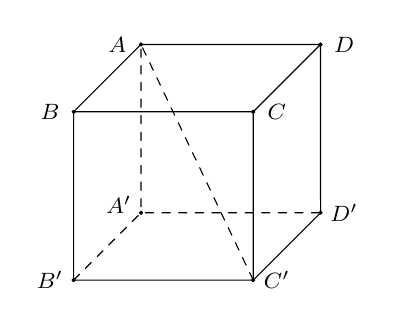
\begin{tikzpicture}[scale=0.57, font=\footnotesize, line join=round, line cap=round, >=stealth]
			\path
			(0,0) coordinate (B) 
			(4,0) coordinate (C) 
			(1.5,1.5) coordinate (A) 
			(A)+(4,0) coordinate (D);
			\foreach \x in {A,B,C,D}
			\path (\x)+(0,-3.75) coordinate(\x');
			\draw[dashed] (B')--(A')--(D') (C')--(A)--(A');
			\draw (B')--(C')--(D')--(D)--(A)--(B)--(C)--(D) (C)--(C') (B)--(B');
			\foreach \p/\g in {B/180,C/0,D/0,A/180,B'/180,C'/0,D'/0,A'/160}
			\draw[fill=black] (\p) circle (1pt)node[shift={(\g:.3)}]{$\p$};
	\end{tikzpicture}}
	\loigiai{
		\immini{Đường chéo của một hình lập phương là $d=a \sqrt{3}$ với $a$ là độ dài cạnh hình lập phương.\\
			Dễ thấy rằng hình lập phương $ABCD.A'B'C'D'$ có $AC'$ là đường chéo và cạnh là $AB$.\\
			Do đó $AC'=AB \sqrt{3} \Rightarrow AB=\dfrac{AC'}{\sqrt{3}}=\dfrac{a \sqrt{3}}{\sqrt{3}}=a$.\\
			Vậy thể tích khối lập phương là $V=a^3$.}
		{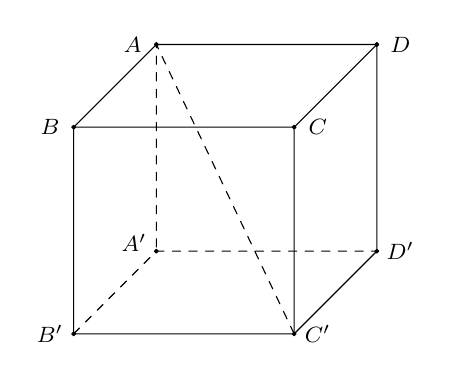
\begin{tikzpicture}[scale=0.7, font=\footnotesize, line join=round, line cap=round, >=stealth]
				\path
				(0,0) coordinate (B) 
				(4,0) coordinate (C) 
				(1.5,1.5) coordinate (A) 
				(A)+(4,0) coordinate (D);
				\foreach \x in {A,B,C,D}
				\path (\x)+(0,-3.75) coordinate(\x');
				\draw[dashed] (B')--(A')--(D') (C')--(A)--(A');
				\draw (B')--(C')--(D')--(D)--(A)--(B)--(C)--(D) (C)--(C') (B)--(B');
				\foreach \p/\g in {B/180,C/0,D/0,A/180,B'/180,C'/0,D'/0,A'/160}
				\draw[fill=black] (\p) circle (1pt)node[shift={(\g:.3)}]{$\p$};
		\end{tikzpicture}}
	}
\end{vd}

\begin{vd}%
	\immini{Tính thể tích của khối lăng trụ đứng $ABCD.A'B'C'D'$ có đáy là hình vuông cạnh $a$, $A'B=2a$.
		\cham{9}
	}{
	\begin{tikzpicture}[scale=0.7, line join=round, line cap=round]
		\tkzDefPoints{0/0/A,-1.3/-1.1/B,2/-1.1/C}
		\coordinate (D) at ($(A)+(C)-(B)$);
		\coordinate (A') at ($(A)+(0,2.5)$);
		\tkzDefPointsBy[translation=from A to A'](B,C,D){B'}{C'}{D'}
		\tkzDrawPolygon(A',B',B,C,D,D')
		\tkzDrawSegments(B',C' C',D' C,C')
		\tkzDrawSegments[dashed](A,B A,D A,A')
		\tkzDrawPoints[fill=black,size=4](A,B,D,C,A',B',C',D')
		\tkzLabelPoints[above](A',D')
		\tkzLabelPoints[below](A,B,C)
		\tkzLabelPoints[left](B')
		\tkzLabelPoints[right](C',D)
\end{tikzpicture}}
	\loigiai{
		\immini{
			Xét tam giác $AA'B$ vuông tại $A$.\\
			suy ra $AA'=\sqrt{A'B^2-AB^2}=\sqrt{(2a)^2-a^2}=a \sqrt{3}$.\\
			$V=AA'.S_{ABCD}=a \sqrt{3} \cdot a^2=a^3 \sqrt{3}$.	
		}
		{
			\begin{tikzpicture}[line cap=round,line join=round, >=stealth,scale=.4]
				\def \xa{-1.5} 
				\def \xb{-1}
				\def \y{4}
				\def \z{4}
				
				\coordinate (A) at (0,0);
				\coordinate (B) at ($(A)+(\xa,\xb)$);
				\coordinate (D) at ($(A)+(\y,0)$);
				\coordinate (C) at ($ (B)+(D)-(A) $);
				\coordinate (B') at ($ (B)+(0,\z) $);
				\coordinate (A') at ($ (A)+(B')-(B) $);
				\coordinate (C') at ($ (C)+(B')-(B) $);
				\coordinate (D') at ($ (D)+(B')-(B) $);
				
				\draw [dashed] (D)--(A)--(A') -- (B) -- (A);
				\draw (B')--(B)--(C)--(D);
				\draw (A') -- (B') -- (C') -- (D')--(A') (C)--(C') (D) --(D') ;
				\tkzDrawPoints(A',B',C',D',A,B,C,D)
				\tkzLabelPoints[right](D)
				\tkzLabelPoints[below right](C)
				\tkzLabelPoint[above](B'){$ B' $}
				\tkzLabelPoint[above](A'){$ A' $}
				\tkzLabelPoint[above](C'){$ C' $}
				\tkzLabelPoint[above](D'){$ D' $}
				\tkzLabelPoints[above right](A)
				\tkzLabelPoints[below left](B)
			\end{tikzpicture}	
		}	
	}
\end{vd}

\begin{vd}
	\immini{Cho lăng trụ tứ giác đều $ABCD.A'B'C'D'$ có cạnh đáy bằng $a$. Góc giữa đường chéo với đáy bằng $60^\circ$. Tính thể tích khối lăng trụ này theo $a$.
		\cham{8}

	}{
		\begin{tikzpicture}[scale=.4]
			\tkzDefPoints{0/0/D, 6/0/C, 8/2/B,2/2/A,0/5/z}
			\coordinate (A') at ($(A)+(z)$);
			\coordinate (B') at ($(B)+(z)$);
			\coordinate (C') at ($(C)+(z)$);
			\coordinate (D') at ($(D)+(z)$);
			\tkzDrawPolygon(A',B',C',D')
			\tkzDrawPoints[size=2,fill=black](A,B,C,D,A',B',C',D')
			\tkzDrawSegments(C,B C,D B,B' C,C' D,D')
			\tkzDrawSegments[dashed](A,B A,D A,A' A,C' A,C)
			\tkzLabelPoints[above](B',D',A')
			\tkzLabelPoints[below](C)
			\tkzLabelPoints[left](A,D)
			\tkzLabelPoints[right](B,C')
	\end{tikzpicture}}
\end{vd}
\begin{vd}
	\immini{Khối hộp chữ nhật $ABCD.A'B'C'D'$ có độ dài $AD$; $AD'$; $AC'$ lần lượt là $1$; $2$; $3$. Tính thể tích $V$ của khối chóp $A.A'B'C'D'$.
		\cham{10}
		
	}{
		\begin{tikzpicture}[scale=.4]
			\tkzDefPoints{0/0/D, 7/0/C, 9/2/B,2/2/A,0/4/z}
			\coordinate (A') at ($(A)+(z)$);
			\coordinate (B') at ($(B)+(z)$);
			\coordinate (C') at ($(C)+(z)$);
			\coordinate (D') at ($(D)+(z)$);
			\tkzDrawPolygon(A',B',C',D')
			\tkzDrawPoints[size=2,fill=black](A,B,C,D,A',B',C',D')
			\tkzDrawSegments(C,B C,D B,B' C,C' D,D')
			\tkzDrawSegments[dashed](A,B A,D A,A' A,C' A,D')
			\tkzLabelPoints[above](B',D',A')
			\tkzLabelPoints[below](C)
			\tkzLabelPoints[left](A,D)
			\tkzLabelPoints[right](B,C')
	\end{tikzpicture}}
\end{vd}

\begin{dang}{Tính thể tích khối chóp}
\end{dang}

\begin{vd}%[2H1Y3-2]
\immini{Cho hình chóp tứ giác $S.ABCD$ có đáy là hình vuông cạnh $a,$ cạnh bên $SA$ vuông góc với đáy và $SA=a\sqrt{3}.$ Tính thể tích $V$ của khối chóp $S.ABCD.$}{
\begin{tikzpicture}[scale=0.5, line join=round, line cap=round]
	\tkzDefPoints{0/0/A,-1.3/-1.6/B,2.5/-1.6/C}
	\coordinate (D) at ($(A)+(C)-(B)$);
	\coordinate (S) at ($(A)+(0,3)$);
	\tkzDrawPolygon(S,B,C,D)
	\tkzDrawSegments(S,C)
	\tkzDrawSegments[dashed](A,S A,B A,D)
	\tkzDrawPoints[fill=black,size=4](D,C,A,B,S)
	\tkzLabelPoints[above](S)
	\tkzLabelPoints[below](A,B,C)
	\tkzLabelPoints[right](D)
\end{tikzpicture}}
\end{vd}

\begin{vd}%[2H1B3-2]
	\immini{Cho hình chóp $S.ABCD$ có đáy $ABCD$ là hình thang vuông tại $A$ và $B$, $AB=BC=\dfrac{AD}{2}=a$. Tam giác $SAB$ đều và nằm trong mặt phẳng vuông góc với đáy. Tính thể tích $V$ của khối chóp $S.ACD$.
	\cham{8}}{
		\begin{tikzpicture}[line cap=round,line join=round,>=stealth,x=1.0cm,y=1.0cm, scale=0.57, thick]
			\tkzDefPoint(0,0){A}
			\def\h{3}
			\def\a{2}
			\tkzDefShiftPoint[A](0:3*\a){D}
			\tkzDefShiftPoint[A](-150:2*\a){B}
			\tkzDefShiftPoint[B](0:1.5*\a){C}
			\coordinate (H) at ($(A)!0.5!(B)$);
			\tkzDefShiftPoint[H](90:1.5*\h){S}
			\tkzDrawSegments[dashed](A,D A,B A,C H,S S,A)
			\tkzDrawSegments(S,B B,C S,C S,D C,D)
			\tkzDrawPoints[size=1pt](A,B,C,D,H,S)
			\pgfresetboundingbox
			\tkzLabelPoints[above](S,A)
			\tkzLabelPoints[below](D,C,B)
			\tkzLabelPoints[left](H)
			\tkzMarkRightAngles(A,H,S A,B,C)
	\end{tikzpicture}}
	\loigiai{
		\immini{
			Gọi $H$ là trung điểm $AB\Rightarrow SH\perp AB$ (vì tam giác $SAB$ đều) và $SH=\dfrac{a\sqrt{3}}{2}$.\\
			Diện tích hình thang $ABCD$ là $\dfrac{3a^{2}}{2}$.\\
			Diện tích tam giác $ABC$ là $\dfrac{a^{2}}{2}\Rightarrow$ diện tích tam giác $ACD=a^{2}\Rightarrow V_{S.ACD}=\dfrac{1}{3}.\dfrac{a\sqrt{3}}{2}.a^{2}=\dfrac{a^{3}\sqrt{3}}{6}$.
		}{
			\hspace*{1cm}
			\begin{tikzpicture}[line cap=round,line join=round,>=stealth,x=1.0cm,y=1.0cm, scale=0.7, thick]
				\tkzDefPoint(0,0){A}
				\def\h{3}
				\def\a{2}
				\tkzDefShiftPoint[A](0:3*\a){D}
				\tkzDefShiftPoint[A](-150:2*\a){B}
				\tkzDefShiftPoint[B](0:1.5*\a){C}
				\coordinate (H) at ($(A)!0.5!(B)$);
				\tkzDefShiftPoint[H](90:1.5*\h){S}
				\tkzDrawSegments[dashed](A,D A,B A,C H,S S,A)
				\tkzDrawSegments(S,B B,C S,C S,D C,D)
				\tkzDrawPoints[size=1pt](A,B,C,D,H,S)
				\pgfresetboundingbox
				\tkzLabelPoints[above](S,A)
				\tkzLabelPoints[below](D,C,B)
				\tkzLabelPoints[left](H)
				\tkzMarkRightAngles(A,H,S A,B,C)
			\end{tikzpicture}
		}
	}
\end{vd}

\begin{vd}%[1H2K7-2]
	\immini{Cho khối chóp đều $S . A B C D$ có đáy $A B C D$ là hình vuông cạnh bằng $a$, góc giữa đường thẳng $S A$ và mặt phẳng $(A B C D)$ bằng $60^{\circ}$. Tính theo $a$ thể tích khối chóp $S . A B C D$.
		\cham{5}
	}{
	\begin{tikzpicture}[scale=0.7, font=\footnotesize, line join=round, line cap=round,>=stealth]
		\path
		(0,0) coordinate (A)
		(-1.9,-1.6)coordinate (B)
		(1.6,-1.6)coordinate (C)
		($(A)+(C)-(B)$)coordinate (D)
		($(A)!0.5!(C)$)coordinate (O)
		($(O)+(0,3)$) coordinate (S)
		;
		\draw (S)--(B)--(C)--(D)--cycle (S)--(C);
		\draw[dashed] (O)--(S)--(A)--(D) (C)--(A)--(B)--(D);
		\foreach \p/\q in {S/90,A/-100,B/-90,C/-90,D/0,O/-90}
		\fill[black] (\p) circle (1.0pt)node[shift={(\q:3mm)}]{$\p$};
		\draw pic[draw=black,angle radius=0.2cm] {right angle = S--O--A}; 
		\draw pic[draw=black,angle radius=0.2cm] {right angle = S--O--D}; 
\end{tikzpicture}}
	\loigiai{
		\immini{
			Gọi $O$ là giao điễm của $A C$ và $B D$ thì $S O \perp(A B C D)$ và góc giữa $S A$ và $(A B C D)$ bằng góc $S A O$ bằng $60^{\circ}$.\\
			Xét tam giác $S A O$ vuông tại $O$, có $A O=\dfrac{a \sqrt{2}}{2}$ và $\widehat{S A O}=60^{\circ}$.\\
			Khi đó $S O=A O \cdot \tan \widehat{S A O}=\dfrac{a \sqrt{2}}{2} \cdot \tan 60^{\circ}=\dfrac{a \sqrt{6}}{2}$.\\
			Do đó, $V_{S . A B C D}=\dfrac{1}{3} \cdot S_{A B C D} \cdot S O=\dfrac{1}{3} \cdot a^2 \cdot \dfrac{a \sqrt{6}}{2}=\dfrac{a^3 \sqrt{6}}{6}$.
		}{
			\begin{tikzpicture}[scale=1, font=\footnotesize, line join=round, line cap=round,>=stealth]
				\path
				(0,0) coordinate (A)
				(-1.9,-1.6)coordinate (B)
				(1.6,-1.6)coordinate (C)
				($(A)+(C)-(B)$)coordinate (D)
				($(A)!0.5!(C)$)coordinate (O)
				($(O)+(0,3.5)$) coordinate (S)
				;
				\draw (S)--(B)--(C)--(D)--cycle (S)--(C);
				\draw[dashed] (O)--(S)--(A)--(D) (C)--(A)--(B)--(D);
				\foreach \p/\q in {S/90,A/-100,B/-90,C/-90,D/0,O/-90}
				\fill[black] (\p) circle (1.0pt)node[shift={(\q:3mm)}]{$\p$};
				\draw pic[draw=black,angle radius=0.2cm] {right angle = S--O--A}; 
				\draw pic[draw=black,angle radius=0.2cm] {right angle = S--O--D}; 
			\end{tikzpicture}
		}
		
	}
\end{vd}
\dongcham{7}
\begin{vd}%[2H1B3]
	\immini{Cho hình chóp $ S.ABCD $ có đáy $ ABCD $ là hình chữ nhật, $ AB = 2a, AD = a $. Hình chiếu của $ S $ lên đáy là trung điểm $ H $ của cạnh $ AB $, góc tạo bởi $ SC $ và đáy là $ 45^{\circ} $. Tính thể tích khối chóp $ S.ABCD $.
	\cham{7}}{
	\begin{tikzpicture}
		\tkzDefPoint(0,0){A}
		\tkzDefShiftPoint[A](0:3){D}
		\tkzDefShiftPoint[A](-150:2){B}
		\tkzDefShiftPoint[B](0:3){C}
		\tkzDefMidPoint(A,B)
		\tkzGetPoint{H}
		\tkzDefShiftPoint[H](90:3){S}
		
		\tkzDrawPoints(S,A,B,C,D,H)
		\tkzLabelPoints(A,B,C,D)
		\tkzLabelPoints[above left](H)
		\tkzLabelPoints[above](S)
		
		\tkzDrawSegments[dashed](S,A A,D A,B S,H H,C)
		\tkzDrawSegments(S,D S,C S,B D,C C,B)
		%\tkzMarkAngle[fill= black!10,arc = l, size = 0.5cm](S,C,H)
\end{tikzpicture}}
	\loigiai{
		\immini{	
			Ta có $ \widehat{[SC,(ABCD)]} = \widehat{SCH} = 45^{\circ} $.	\\
			Ta có $ SH = HC = \sqrt{BH^2 + BC^2 } = a \sqrt{2} $.\\
			Thể tích $ V_{S.ABCD} = \dfrac{2\sqrt{2}a^3}{3} $.
		}{
			\begin{tikzpicture}
				\tkzDefPoint(0,0){A}
				\tkzDefShiftPoint[A](0:3){D}
				\tkzDefShiftPoint[A](-150:2){B}
				\tkzDefShiftPoint[B](0:3){C}
				\tkzDefMidPoint(A,B)
				\tkzGetPoint{H}
				\tkzDefShiftPoint[H](90:3){S}
				
				\tkzDrawPoints(S,A,B,C,D,H)
				\tkzLabelPoints(A,B,C,D)
				\tkzLabelPoints[above left](H)
				\tkzLabelPoints[above](S)
				
				\tkzDrawSegments[dashed](S,A A,D A,B S,H H,C)
				\tkzDrawSegments(S,D S,C S,B D,C C,B)
				%\tkzMarkAngle[fill= black!10,arc = l, size = 0.5cm](S,C,H)
			\end{tikzpicture}
		}
	}		
\end{vd}
\dongcham{3}
\begin{vd}
	\immini{Tính thể tích khối tứ diện đều cạnh bằng $2a$.
		\cham{9}
	}{
		\begin{tikzpicture}[scale=0.8]
			\tikzset{label style/.style={font=\footnotesize}}
			\tkzDefPoints{0/0/A,1/-2/B,5/0/C}
			\tkzCentroid(A,B,C)\tkzGetPoint{G}
			\coordinate (D) at ($(G)+(0,3)$);
			\coordinate (M) at ($(A)!0.5!(B)$);
			\coordinate (N) at ($(B)!0.5!(C)$);
			\tkzDrawPoints[size=2,fill=black](A,B,C,D,M,N,G)
			\tkzDrawSegments(D,A D,B D,C A,B B,C)
			\tkzDrawSegments[dashed](A,C D,G A,N C,M)
			\tkzLabelPoints[above](D)
			\tkzLabelPoints[left](A,M)
			\tkzLabelPoints[right](C)
			\tkzLabelPoints[below](B,G,N)
	\end{tikzpicture}}
\end{vd}
\dongcham{4}
\begin{vd}
	\immini{Cho hình chóp $S.ABC$ có đáy $ABC$ là tam giác đều cạnh $a$, cạnh bên $SA$ vuông góc với đáy $(ABC)$. Biết góc tạo vởi hai mặt phẳng $(SBC)$ và $(ABC)$ bằng $60^\circ$, tính thể tích $V$ của khối chóp $S.ABC$.
		\cham{6}
	}{\hspace{1cm}
		\begin{tikzpicture}[smooth,font=\footnotesize,scale=0.8]
			\path
			(0,0) coordinate (A)
			(1,-1.5) coordinate (B)
			(5,0) coordinate (C);
			\coordinate (S) at ($(A)+(0,2.5)$);
			\coordinate (M) at ($(B)!0.5!(C)$);
			\draw (S)--(A)--(B)--(C) (B)--(S)--(C) (S)--(M);
			\draw[dashed] (A)--(C) (A)--(M);
			\foreach \x/\g in {A/180,B/-90,C/0,S/90,M/-40} \draw [fill=black] (\x) circle (.05) + (\g:.3) node{$\x$};
			\begin{scope}
				\clip (S)--(M)--(A);
				\draw[double] (M) circle(0.7cm);
			\end{scope}
	\end{tikzpicture}}
\end{vd}
\dongcham{4}
\begin{dang}{Tính thể tích khối chóp cụt đều}
	\begin{enumerate}[\iconCH]
		\item \indamm{Phương pháp:}
		\begin{itemize}
			\item Tính diện tích hai đáy (lớn, bé) $S$, $S'$ và độ dài đường cao $h$ của khối chóp cụt đều;
			\item Thay vào công thức $V\dfrac{1}{3}\cdot h\cdot (S+S'+\sqrt{S\cdot S'})$.
		\end{itemize}
	\end{enumerate}
	
\end{dang}

\begin{vd}%[1H2B7-2]
	\immini{Tính thể tích của khối chóp cụt tam giác đều $ABC.A'B'C'$ có chiều cao bằng $3a$, $AB=4a$, $A'B'=a$.
	\cham{7}}{
	\begin{tikzpicture}[scale=0.85, line join=round, line cap=round]
		\tkzDefPoints{0/0/A,1.2/-1.6/B,4.5/0/C}
		\tkzCentroid(A,B,C)\tkzGetPoint{G}
		\coordinate (S) at ($(G)+(0,3.5)$);
		\coordinate (M) at ($(B)!1/2!(C)$);
		\coordinate (A') at ($(S)!1/2!(A)$);
		\coordinate (B') at ($(S)!1/2!(B)$);
		\coordinate (C') at ($(S)!1/2!(C)$);
		\tkzDrawPolygon(A,B,B',A')
		\tkzDrawPolygon(B,C,C',B')
		\tkzDrawSegments(A',C')
		\tkzDrawSegments[dashed](A,C)
		\tkzDrawPoints[fill=black,size=4](A,B,C,A',B',C')
		\tkzLabelPoints[above](A',B',C')
		\tkzLabelPoints[below](B)
		\tkzLabelPoints[left](A)
		\tkzLabelPoints[right](C)
\end{tikzpicture}}
	\loigiai{
		Diện tích tam giác đều $ABC: S=\dfrac{AB^2 \sqrt{3}}{4}=\dfrac{(4a)^2 \sqrt{3}}{4}=4a^2 \sqrt{3}$.\\
		Diện tích tam giác đều $A'B'C': S'=\dfrac{A'B'^2 \sqrt{3}}{4}=\dfrac{a^2 \sqrt{3}}{4}$.\\
		Thể tích khối chóp cụt
		$$
		V=\dfrac{1}{3} \cdot 3a \cdot\left(4 a^2 \sqrt{3}+\sqrt{4 a^2 \sqrt{3} \cdot \dfrac{a^2 \sqrt{3}}{4}}+\dfrac{a^2 \sqrt{3}}{4}\right)=\dfrac{21 a^3 \sqrt{3}}{4}.$$		
	}
\end{vd}
\dongcham{4}
\begin{vd}%[1H2B7-2]
	\immini{Tính thể tích một cái sọt đựng đồ có đạng hình chóp cụt tứ giác đều, đáy lớn có cạnh bằng $80$ cm, đáy nhỏ có cạnh bằng $40$ cm và cạnh bên bằng $80$ cm.
	\cham{4}}{
	\begin{tikzpicture}[scale=1.5,>=stealth,line join=round,line cap=round,font=\footnotesize]
		\path
		(0,0)coordinate(A)
		(-130:1)coordinate(B)
		(2,0)coordinate(D)
		($(D)-(A)+(B)$)coordinate(C)
		(intersection of A--C and B--D)coordinate(O)
		($(O)+(-90:2)$)coordinate(S)
		($(A)!1/2!(S)$)coordinate(A')
		($(B)!1/2!(S)$)coordinate(B')
		($(C)!1/2!(S)$)coordinate(C')
		($(D)!1/2!(S)$)coordinate(D')
		($(B')!1/2!(C')$)coordinate(M)
		;
		\draw(A)--(B)--(B')--(C')--(D')--(D)--cycle(B)--(C)--(D) (C)--(C');
		\draw[dashed](B')--(A')--(D')(A)--(A');
\end{tikzpicture}}
	\loigiai{
		\immini{Ta có $OC=40 \sqrt{2}$, $OC'=20 \sqrt{2}$, suy ra $CH=20 \sqrt{2}$.\\
			Trong tam giác vuông $C'CH$, ta có
			$C'H=\sqrt{CC'^2-CH^2}=20 \sqrt{14}$.\\
			Nên $OO'=C'H=20 \sqrt{14}$.\\
			Thể tích của cái sọt đựng đồ là
			$$
			V=\dfrac{1}{3} \cdot 20 \sqrt{14} \cdot(6400+\sqrt{6400 \cdot 1600}+1600) \approx 279\,377{,}08 \mathrm{~cm}^3 .
			$$}
		{\begin{tikzpicture}[>=stealth,line join=round,line cap=round,font=\footnotesize,scale=0.7]
				\path (0,0) coordinate (D)
				(6,0) coordinate (C)
				(-3,-2) coordinate (A)
				($(C)-(D)+(A)$) coordinate (B)
				($(A)!1/2!(C)$) coordinate (O)
				($(O)+(0,6)$) coordinate (S)
				($(A)!.6!(S)$) coordinate (A')
				($(B)!.6!(S)$) coordinate (B')
				($(C)!.6!(S)$) coordinate (C')
				($(D)!.6!(S)$) coordinate (D')
				($(A')!.5!(C')$) coordinate (O')
				($(O)!.42!(C)$) coordinate (H)
				; 
				\draw (C')--(A')--(A)--(B)--(C)--(C')--(D')--(A')--(B')--(C') (B)--(B')--(D')
				;
				\draw[dashed] (D)--(C)--(A)--(D) (B)--(D)--(D') (O)--(O') (C')--(H) 
				;
				\foreach \p/\r in {A/180,B/-70,C/0,D/150,A'/180,B'/-30,C'/10,D'/150,O/-90,O'/80,H/-90}
				\fill (\p) circle (1.5pt) node[scale=.7,shift={(\r:2.5mm)}]{$\p$};
		\end{tikzpicture}}
	}
\end{vd}
\dongcham{3}

